%-------------------------------------------------------------------------------
%-------------------------------------------------------------------------------
%-------------------------------------------------------------------------------
\chapter{Moyennisation}
%-------------------------------------------------------------------------------
%-------------------------------------------------------------------------------
%-------------------------------------------------------------------------------

Les 3 parties de ce devoir sont indépendantes.
\begin{itemize}
    \item La première partie porte sur de l'algorithmique simple de première année
    \item La deuxième partie étudie une modélisation de chimie, elle correspond au programme du second semestre de sup.
    \item La troisième partie reprend des calculs d'algorithmes en introduisant quelques calculs de complexité.
\end{itemize}

\medskip

Il est rappelé qu'il est toujours possible d'utiliser une fonction demandée dans une question pour l'écriture d'autres solutions {\bf même si on n'a pas écrit cette fonction.}

%-------------------------------------------------------------------------------
%-------------------------------------------------------------------------------
%-------------------------------------------------------------------------------
\section{Droites d'approximations} 
%-------------------------------------------------------------------------------
%-------------------------------------------------------------------------------
%-------------------------------------------------------------------------------
\subsection{Fonctions classiques} 
%-------------------------------------------------------------------------------
%-------------------------------------------------------------------------------
\begin{Exercise}[title = Moyenne]
\it Écrire une fonction \type{moyenne(X)} qui calcule la moyenne des termes de la liste $X$ :

$\displaystyle \type{moyenne(X)} = \frac 1n \sum_{i=0}^n \type{X[i]}$ avec $n = \type{len(X)}$.
\end{Exercise}
%-------------------------------------------------------------------------------
\begin{Answer}
\begin{lstlisting}
def moyenne(X):
    n = len(X)
    somme = 0
    for i in range(n):
        somme = somme + X[i]
    return somme/n
\end{lstlisting}
\end{Answer}
%-------------------------------------------------------------------------------
%-------------------------------------------------------------------------------
\bigskip

La {\bf variance} d'une liste est définie par $\displaystyle \text{var}(X) =  \frac 1n \sum_{i=0}^n \bigl(\type{X[i]} -m_X\bigr)^2$ avec $m_X$ égal à la moyenne de la liste et $n = \type{len(X)}$.
%-------------------------------------------------------------------------------
%-------------------------------------------------------------------------------
\begin{Exercise}[title = Variance]
\it Écrire une fonction \type{var(X)} qui calcule la variance de la liste $X$.
\end{Exercise}
%-------------------------------------------------------------------------------
\begin{Answer}
\begin{lstlisting}
def var(X):
    n = len(X)
    mX = moyenne(X)
    somme = 0
    for i in range(n):
        somme = somme + (X[i] - mX)**2
    return somme/n
\end{lstlisting}
\end{Answer}
%-------------------------------------------------------------------------------
%-------------------------------------------------------------------------------
\subsection{Droite de régression} 
%-------------------------------------------------------------------------------
%-------------------------------------------------------------------------------
Si $X$ et $Y$ sont deux listes de même longueur, la {\bf covariance} de $X$ est $Y$ est 

$\displaystyle \text{cov}(X, Y) =  \frac 1n \sum_{i=0}^n \bigl(\type{X[i]} -m_X\bigr)\bigl(\type{Y[i]} -m_Y\bigr)$ avec $m_X$ égal à la moyenne de la liste $X$, $m_Y$ égal à la moyenne de la liste $Y$ et $n$ est la longueur commune de $X$ et de $Y$.

On pourra noter que $\text{var}(X) = \text{cov}(X, X)$
%-------------------------------------------------------------------------------
%-------------------------------------------------------------------------------
\begin{Exercise}[title = Covariance]
\it Écrire une fonction \type{cov(X, Y)} qui calcule la covariance des listes $X$ et $Y$.
\end{Exercise}
%-------------------------------------------------------------------------------
\begin{Answer}
\begin{lstlisting}
def cov(X, Y):
    n = len(X)
    mX = moyenne(X)
    mY = moyenne(Y)
    somme = 0
    for i in range(n):
        somme = somme + (X[i] - mX)*(Y[i] - mY)
    return somme/n
\end{lstlisting}
\end{Answer}
%-------------------------------------------------------------------------------
%-------------------------------------------------------------------------------
\bigskip

Si $X$ et $Y$ sont deux listes de même longueur, leur {\bf produit} est la liste $Z$ de même longueur telle que \type{Z[i] = X[i]*Y[i]} pour tout indice $i$ compris entre 0 et $n-1$.

%-------------------------------------------------------------------------------
%-------------------------------------------------------------------------------
\begin{Exercise}[title = Produit]
\it Écrire une fonction \type{produit(X, Y)} qui calcule la liste produit des listes $X$ et $Y$.
\end{Exercise}
%-------------------------------------------------------------------------------
\begin{Answer}
\begin{lstlisting}
def produit(X, Y):
    n = len(X)
    Z = [0]*n
    for i in range(n):
        Z[i] = X[i]*Y[i]
    return Z
\end{lstlisting}
\end{Answer}
%-------------------------------------------------------------------------------
%-------------------------------------------------------------------------------
\bigskip

On admet que, si $Z$ est le produit des listes $X$ et $Y$, alors $\text{cov}(X, Y) = m_Z - m_X.m_Y$ où $m_X$, $m_Y$ et $m_Z$ sont les moyennes respectivement des listes $X$, $Y$ et $Z$.
%-------------------------------------------------------------------------------
%-------------------------------------------------------------------------------
\begin{Exercise}[title = Calcul alternatif]
\it Écrire une fonction \type{cov(X, Y)} qui calcule la covariance des listes $X$ et $Y$ sans utiliser de boucles mais en employant les fonctions \type{moyenne} et \type{produit}.
\end{Exercise}
%-------------------------------------------------------------------------------
\begin{Answer}
\begin{lstlisting}
def cov(X, Y):
    n = len(X)
    mX = moyenne(X)
    mY = moyenne(Y)
    Z = produit(X, Y)
    mZ = moyenne(Z)
    return mZ - mX*mY
\end{lstlisting}
\newpage
\end{Answer}
%-------------------------------------------------------------------------------
%-------------------------------------------------------------------------------
\bigskip

On admet que, $X$ et $Y$ sont deux listes de même longueur, alors la {\bf droite de régression} approchant $Y$ par rapport à $X$ est la droite d'équation $y = ax+b$ avec $m_Y = a.m_X + b$ et $a.\text{var}(X)=\text{cov}(X, Y)$.
%-------------------------------------------------------------------------------
%-------------------------------------------------------------------------------
\begin{Exercise}[title = Droite de régression]
\it Écrire une fonction \type{regression(X, Y)} qui calcule les coefficients$a$ et $b$ de la droite de régression de $X$ à $Y$.
\end{Exercise}
%-------------------------------------------------------------------------------
\begin{Answer}
\begin{lstlisting}
def regression(X, Y):
    a = cov(X, Y)/var(X)
    b = moyenne(Y) - a*moyenne(X)
    return a, b
\end{lstlisting}
\end{Answer}
%-------------------------------------------------------------------------------
%-------------------------------------------------------------------------------
\subsection{Méthode de Wald} 
%-------------------------------------------------------------------------------
%-------------------------------------------------------------------------------
Il existe d'autres droites qui permettent d'approcher les variations de $Y$ par rapport à $X$.

La méthode de Wald consiste à

\begin{itemize}
\item séparer les listes en deux parties quasi-égales : $X$ donne $Xg$ et $Xd$ et $Y$ donne $Yg$ et $Yd$,

\item calculer les moyennes des quatre parties,

\item déterminer la droite $y=ax+b$ telle que 

\type{moyenne(Yg) = a*moyenne(Xg) + b} et 
\type{moyenne(Yd) = a*moyenne(Xd) + b}
\end{itemize}

\medskip

On suppose que la liste $X=[x_0, x_1,x_2,\ldots,x_{n-1}]$ est croissante.

Si $X$ comporte $n$ éléments et si $m=\left\lfloor\frac n 2\right\rfloor$ (\type{m = n//2}), on définit 

$Xg=[x_0, x_1,x_2,\ldots,x_{m-1}]$ et $Xd=[x_m, x_{m+1}, \ldots,x_{n-1}]$.

On sépare alors $Y$ selon le même indice :  \type{Yg = Y[0 : m]} et \type{Yd = Y[m : n]}. 

Ainsi les sous-suites de droite ont autant d'éléments que les sous-suites de gauche ou un de plus.
%-------------------------------------------------------------------------------
%-------------------------------------------------------------------------------
\begin{Exercise}[title = Séparation]
\it Écrire en Python une fonction \type{separer(U)} qui détermine les deux listes définies en séparant comme ci-dessus.
\end{Exercise}
%-------------------------------------------------------------------------------
\begin{Answer}
\begin{lstlisting}
def separer2(U):
    n = len(U)
    m = n//2
    return U[ : m], U[m : ]
\end{lstlisting}
\end{Answer}
%-------------------------------------------------------------------------------
%-------------------------------------------------------------------------------
\begin{Exercise}[title = Droite de Wald]
\it Écrire en Python une fonction \type{wald(X,Y)} qui, à partir de deux listes de même longueur \type{X} et \type{Y}, calcule le couple \type{(a,b)} des coefficients $a$ et $b$ déterminés ci-dessus.
\end{Exercise}
%-------------------------------------------------------------------------------
\begin{Answer}
\begin{lstlisting}
def wald(X, Y):
    Xg, Xd = separer2(X)
    Yg, Yd = separer2(Y)
    mXg = moyenne(Xg)
    mXd = moyenne(Xd)
    mYg = moyenne(Yg)
    mYd = moyenne(Yd)
    a = (mYd - mYg)/(mXd - mXg)
    b = mYd - a*mYd
    return a, b
\end{lstlisting}
\end{Answer}
%-------------------------------------------------------------------------------
%-------------------------------------------------------------------------------
\bigskip

La troisième partie donnera d'autres calculs de droites.
%-------------------------------------------------------------------------------
\newpage
%-------------------------------------------------------------------------------
%-------------------------------------------------------------------------------
\section{Phosgène} 
%-------------------------------------------------------------------------------
%-------------------------------------------------------------------------------
%-------------------------------------------------------------------------------
Le phosgène COCl${}_2$ est gaz qui a servi de gaz de combat pendant la première guerre mondiale. 

Il est utilisé maintenant dans de nombreuses synthèses, en particulier des isocyanates.

A haute température il se décompose selon COCl${}_2 \longrightarrow $ CO + Cl${}_2$.

L'étude du mécanisme indique que la réaction est d'ordre 1 en COCl${}_2$ et d'ordre $\frac12$ en Cl${}_2$.

On note $y(t)$ la concentration en Cl${}_2$ au temps $t$.

La concentration de phosgène introduite dans le gaz n'est pas constante : elle est donnée par une loi $\alpha(t)$.
On aboutit alors à l'équation différentielle
    \[y'(t) = k\bigl(\alpha(t)-y\bigr) \sqrt{y}=\varphi(y, t)\leqno(E)\]
%-------------------------------------------------------------------------------
%-------------------------------------------------------------------------------
\subsection{Premières fonctions} 
%-------------------------------------------------------------------------------
%-------------------------------------------------------------------------------
\begin{Exercise}\it
Écrire une fonction \type{listeT(a, b, n)} qui calcule une liste de longueur $n$ dont les valeurs sont équiréparties entre $a$ et $b$.
\end{Exercise}
%-------------------------------------------------------------------------------
\begin{Answer}
\begin{lstlisting}
def listeT(a, b, n):
    pas = (b-a)/(n-1)
    T = [0]*n
    for k in range(n):
        T[k] = a + k*pas 
    return T
\end{lstlisting}
\end{Answer}
%-------------------------------------------------------------------------------
\smallskip
\type{listeT(1, 3, 5)} doit renvoyer \type{[1.0, 1.5, 2.0, 2.5, 3.0]}.

On remarquera que le pas est $\frac{b-a}{n-1}$.

\bigskip

On suppose que la fonction $\alpha$ est définie par la formule
\[\alpha(t) = \left\{\begin{matrix}\alpha_0 + ct&\text{pour }t < T_s\\ \alpha_0 + c.T_s&\text{pour }t \ge T_s
\end{matrix}\right.
\]
Les constantes $k = 2,4.10^{-2}$ mole${}^{-1/2}$ L${}^{1/2}$ s${}^{-1}$, $\alpha_0 = 10^{-8}$  mole L${}^{-1}$, $c = 0.2$ L${}^{-1}$ s${}^{-1}$ 

et $T_s = 10$ s (le seuil) sont données par les variables globales
\begin{lstlisting}
k = 2.4e-2 
alpha0 = 1e-8
c = 0.2
T_s = 10
\end{lstlisting}
On utilisera les variables dans les fonctions à écrire plutôt que leurs valeurs.
%-------------------------------------------------------------------------------
%-------------------------------------------------------------------------------
\begin{Exercise}\it
Écrire la fonction \type{alpha(t)} qui calcule la valeur de $\alpha(t)$ en fonction du temps $t$.
\end{Exercise}
%-------------------------------------------------------------------------------
\begin{Answer}
\begin{lstlisting}
def phi(x, t):
    return k*(alpha*t - x)*x**0.5
\end{lstlisting}
\end{Answer}
%-------------------------------------------------------------------------------
%-------------------------------------------------------------------------------
\begin{Exercise}\it
Écrire la fonction \type{phi(x, t)} qui définit l'équation $(E)$ ; elle traduit $\varphi$ en python.
\end{Exercise}
%-------------------------------------------------------------------------------
\begin{Answer}
\begin{lstlisting}
def alpha(t):
    if t < Ts:
        return alpha0 + c*t
    else:
        return alpha0 + c*Ts
\end{lstlisting}
\newpage
\end{Answer}
%-------------------------------------------------------------------------------
\newpage
%-------------------------------------------------------------------------------
\subsection{Méthode d'Euler} 
%-------------------------------------------------------------------------------
%-------------------------------------------------------------------------------
On rappelle que la résolution de l'équation nécessite
\begin{itemize}
    \item la fonction \type{phi(y, t)},
    \item une liste \type{T} de valeurs de $t$,
    \item la condition initiale \type{y0} qui est la valeur de la solution recherchée au temps \type{T[0]}.
\end{itemize}
La solution sera donnée sous la forme d'une liste \type{Y} de même taille que \type{T} et telle que \type{Y[i]} approche la valeur de la solution en \type{T[i]}.
%-------------------------------------------------------------------------------
%-------------------------------------------------------------------------------
\begin{Exercise}\it
Écrire la fonction \type{euler(phi, y0, T)} qui calcule une solution en utilisant la méthode d'Euler.
\end{Exercise}
%-------------------------------------------------------------------------------
\begin{Answer}
\begin{lstlisting}
def euler(phi, y0, T):
    n = len(T)
    Y = [0]*n
    Y[0] = y0 
    for i in range(n-1): 
        pas = T[i+1] - T[i]
        pente = phi(Y[i], T[i])  
        Y[i+1] = Y[i] + pas*pente
    return Y
\end{lstlisting}
\end{Answer}
%-------------------------------------------------------------------------------
%-------------------------------------------------------------------------------
\begin{Exercise}\it
Donner les instructions qui permettent de calculer une solution sur l'intervalle de temps $[0;200]$ avec une condition initiale $y_0 = \frac 12 \alpha_0$. On choisira une liste de temps avec 1000 points.
\end{Exercise}
%-------------------------------------------------------------------------------
\begin{Answer}
\begin{lstlisting}
y0 = alpha0/2
t_max = 200
n = 1000
T = listeT(0, t_max, n)
Y = euler(phi, y0, T)
\end{lstlisting}
\end{Answer}
%-------------------------------------------------------------------------------
%-------------------------------------------------------------------------------
\begin{Exercise}\it
Pourquoi a-t-on choisi une condition initiale non nulle ? On pourra trouver une solution très simple si $y_0=0$. 
\end{Exercise}
%-------------------------------------------------------------------------------
\begin{Answer}Pour $y_0=0$, une solution est la fonction nulle, on veut voir évoluer le système.
\end{Answer}
%-------------------------------------------------------------------------------
%-------------------------------------------------------------------------------
\subsection{Schéma du point médian} 
%-------------------------------------------------------------------------------
%-------------------------------------------------------------------------------
On suppose dans cette partie que les temps $t_i$ sont tels que le pas $t_{i+1} - t_i$ est constant ; on note $h$ sa valeur. On notera que c'est le cas pour les listes \type{listeT(a, b, n)} où on a $h = \frac{b-a}{n-1}$


On rappelle que le schéma d'Euler consiste, pour une fonction $f$ de classe ${\cal C}^1$, 

 à approcher $f(t_{i+1})$ par $f(t_i) + (t_{i+1} - t_i)f'(t_i) = f(t_i) + hf'(t_i)$.
%-------------------------------------------------------------------------------
%-------------------------------------------------------------------------------
\begin{Exercise}[title = {Des maths simples}]\it
En écrivant un développement limité à l'ordre 2 de $f$ pour calculer $f(t_{i+1})$ en fonction de $f(t_i)$, $f'(t_i)$ et $f''(t_i)$, montrer que l'erreur commise par l'approximation du schéma d'Euler peut s'écrire
\[f(t_{i+1})- f(t_i) - hf'(t_i) = A_2h^2 + o\bigl(h^2\bigr)\]
\end{Exercise}
%-------------------------------------------------------------------------------
\begin{Answer}
$f(t_{i+1})- f(t_i) - hf'(t_i) = \frac{f''(t_i)}2h^2 + o\bigl(h^2\bigr)$
\end{Answer}
%-------------------------------------------------------------------------------
%-------------------------------------------------------------------------------
\begin{Exercise}[title = {Un peu de calcul mathématique}]\it
En écrivant deux développementx limitéx à l'ordre 3 de $f$ pour calculer $f(t_{i+1})$ et $f(t_{i-1})$ en fonction des valeurs en $t_i$, montrer qu'on a
\[f(t_{i+1})- f(t_{i-1}) - 2hf'(t_i) = A_3h^3 + o\bigl(h^3\bigr)\]
On rappelle qu'on a $t_{i-1} - t_i = -h$
\end{Exercise}
%-------------------------------------------------------------------------------
\begin{Answer}
$f(t_{i+1})= f(t_i) + hf'(t_i) + \frac{f''(t_i)}2h^2 + \frac{f^{(3)}(t_i)}6h^3 + o\bigl(h^3\bigr)$

$f(t_{i+1})= f(t_i) - hf'(t_i) + \frac{f''(t_i)}2h^2 - \frac{f^{(3)}(t_i)}6h^3 + o\bigl(h^3\bigr)$

d'où $f(t_{i+1})- f(t_{i-1}) = 2hf'(t_i) + \frac{f^{(3)}(t_i)}3h^3 + o\bigl(h^3\bigr)$.
\end{Answer}
%-------------------------------------------------------------------------------
%-------------------------------------------------------------------------------
\bigskip

Ainsi l'approximation de $f(t_{i+1})$ par $f(t_{i-1}) + 2hf'(t_i)$ semble permettre des calculs plus précis pour des petites valeurs du pas. 

On notera cependant que cette méthode ne peut pas s'appliquer pour évaluer $f(t_1)$.

On propose donc le schéma de calcul suivant pour approcher les valeurs des $f(t_i)$ par $y_i$.

\begin{itemize}
\item On a la valeur de $y_0$.
\item On calcule $y_1$ par le schéma d'Euler : $y_1 = y_0 + hf'(t_0) = y_0 + h\varphi(y_0, t_0)$.
\item Pour $i$ prenant les valeurs de 1 à $n-2$, on calcule 
\item $y_{i+1} = y_{i-1} + 2h\varphi(y_i, t_i)$.
\end{itemize}
%-------------------------------------------------------------------------------
%-------------------------------------------------------------------------------
\begin{Exercise}\it
Écrire la fonction \type{median(phi, y0, T)} qui calcule une solution approchée en utilisant ce schéma.

On devra calculer le pas $h$ {\bf avant} la boucle \type{for} : $h = t_1-t_0$.
\end{Exercise}
%-------------------------------------------------------------------------------
\begin{Answer}
\begin{lstlisting}
def median(phi, y0, T):
    n = len(T)
    Y = [0]*n
    h = T[1] - T[0]
    Y[0] = y0 
    Y[1] = y0 + h*phi(y0, T[0])
    for i in range(2, n-1): 
        pente = phi(Y[i], T[i])  
        Y[i+1] = Y[i-1] + 2*h*pente
    return Y
\end{lstlisting}
\end{Answer}
%-------------------------------------------------------------------------------
%-------------------------------------------------------------------------------

La figure ci-après compare les solutions obtenues par les deux méthodes. On constate une amélioration de l'approximation avec, cependant, une instabilité des valeurs visible autour de $t=200$. Cette instabilité ne permet pas la généralisation de cette méthode.
%-------------------------------------------------------------------------------
\begin{figure}[ht]
\begin{center}
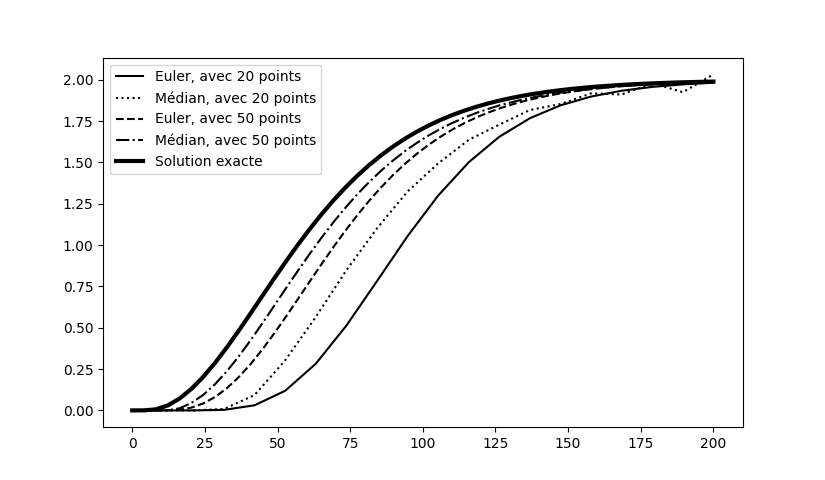
\includegraphics[width=\linewidth]{DS1_PC}
\caption{Solutions comparées}
\end{center}
\end{figure}
%-------------------------------------------------------------------------------
%-------------------------------------------------------------------------------
\subsection{Dépassement} 
%-------------------------------------------------------------------------------
%-------------------------------------------------------------------------------
On demande parfois le moment où la concentration atteint une valeur donnée.

On suppose que la liste \type{Y} est triée par ordre croissant.

On se donne un seuil $s$ strictement compris entre les valeurs extrêmes de la liste \type{Y}, par exemple $s = 1.2$ dans les solutions ci-dessus et on cherche l'indice $i$ tel que \type{Y[i] <= s < Y[i+1]}
%--------------------------------------------------------------------------
% --------------------------------------------------------------------------
\begin{Exercise}\it Écrire une fonction \type{indiceSeuil(Y, s)} qui calcule cet indice.
\end{Exercise}
% --------------------------------------------------------------------------
\begin{Answer} On balaye la liste.
\begin{lstlisting}
def indiceSeuil(Y, k):
    i = 0
    while liste[i+1] <= s:
        i = i+1
    return i
\end{lstlisting}
\newpage
\end{Answer}
%--------------------------------------------------------------------------
% --------------------------------------------------------------------------
\begin{Exercise}\it Modifier en  une fonction \type{tempsSeuil(T, Y, s)} qui renvoie le temps \type{T[i]} où se produit le dépassement.
\end{Exercise}
% --------------------------------------------------------------------------
\begin{Answer} 
\begin{lstlisting}
def tempsSeuil(T, Y, s):
    i = 0
    while liste[i+1] <= s:
        i = i+1
    return T[i]
\end{lstlisting}
\end{Answer}
%--------------------------------------------------------------------------
% --------------------------------------------------------------------------
\medskip

Si on ne suppose pas que le seuil est franchi on peut vouloir cependant avoir un résultat. 
%--------------------------------------------------------------------------
% --------------------------------------------------------------------------
\begin{Exercise}\it Modifier la fonction \type{indiceSeuil(T, Y, s)} pour qu'elle renvoie 
\begin{itemize}
    \item l'indice $i$ tel que \type{Y[i] <= s < Y[i+1]} si cet indice existe,
    \item -1 si on a \type{s < Y[0]},
    \item n-1 si on a \type{Y[n-1] > = s} ($n$ est la longueur de la liste \type{Y}.)
\end{itemize}
\end{Exercise}
% --------------------------------------------------------------------------
\begin{Answer}
\begin{lstlisting}
def indiceSeuil(T, Y, s):
    i = -1
    while i < n-1 and liste[i+1] <= s:
        i = i+1
    return i
\end{lstlisting}
\end{Answer}
%-------------------------------------------------------------------------------
\newpage
%-------------------------------------------------------------------------------
%-------------------------------------------------------------------------------
\section{Médiane} 
%-------------------------------------------------------------------------------
%-------------------------------------------------------------------------------
%-------------------------------------------------------------------------------
On revient à la problématique de la première partie pour rechercher une droite qui approche au mieux un ensemble de points défini par les liste \type{X} et \type{Y} ; pour simplifier les écriture on notera $x_i$ (respectivement $y_i$) la valeur de \type{X[i]} (respectivement de \type{Y[i]}).

La méthode de Wald décrite ci-dessus comporte le calcul des moyennes mais on sait que la moyenne, dans des résultats expérimentaux, peut être est perturbée par la présence de points aberrants.

Un moyen classique de gérer ces points est de considérer la médiane plutôt que la moyenne.

\begin{defin}
La médiane d'une liste de points $U=(u_0u_1, u_2,\ldots,u_{n-1})$ est une valeur qui partage la liste en deux parties quasi- égales. 
\end{defin}
%-------------------------------------------------------------------------------
%-------------------------------------------------------------------------------
\subsection{Listes sans points doubles} 
%-------------------------------------------------------------------------------
%-------------------------------------------------------------------------------
Dans le cas d'une liste de points {\bf distincts} on trie la liste en $(v_0, v_1,\ldots,v_{n-1}$ 

\begin{enumerate}
\item Si $n$ est impair, $n=2p+1$, la médiane est $v_p$ : il y a $p$ éléments qui lui sont strictement inférieurs et $p$ éléments qui lui sont strictement supérieurs.
\item si, $n$ est pair, $n=2p$, la médiane peut être 

$v_{p-1}$ : il y a $p-1$ éléments strictement inférieurs et $p$ éléments strictement supérieurs

ou $v_p$ : il y a $p$ éléments strictement inférieurs et $p-1$ éléments strictement  supérieurs.

On choisira $v_p$ comme médiane dans ce cas.
\end{enumerate}
\medskip

On ne suppose pas que les listes sont triées.
%--------------------------------------------------------------------------
% --------------------------------------------------------------------------
\begin{Exercise}\it Montrer que, pour une liste de points distincts et de longueur $n$, il y a \type{n//2} éléments strictement supérieurs à la médiane et \type{(n-1)//2} éléments strictement inférieurs à la médiane.
\end{Exercise}
% --------------------------------------------------------------------------
\begin{Answer} 
Pour $n=2p$, \type{p = n//2} et \type{p - 1 = (n-1)//2},

pour $n=2p+1$, \type{p = n//2} et \type{p = (n-1)//2}.

On trouve bien les valeurs souhaitées.
\end{Answer}
%--------------------------------------------------------------------------
% --------------------------------------------------------------------------
\medskip

Pour trouver la médiane d'une liste de points distincts il suffit donc de trouver l'élément de la liste qui admet exactement \type{(n-1)//2} éléments strictement inférieurs dans la liste.
%--------------------------------------------------------------------------
% --------------------------------------------------------------------------
\begin{Exercise}\it Écrire une fonction \type{rang(x, L)} qui renvoie le nombre d'éléments de la liste $L$ qui sont strictement inférieurs à $x$. On pourra parcourir la liste et augmenter un compteur pour chaque élément de la liste strictement inférieur à $x$.

Combien de comparaisons sont-elles effectuées ?
\end{Exercise}
% --------------------------------------------------------------------------
\begin{Answer} 
\begin{lstlisting}
def rang(x, L):
    n = len(L)
    compteur = 0
    for i in range(n):
        if liste[i] < x:
            compteur = compteur + 1
    return compteur
\end{lstlisting}
\end{Answer}
%--------------------------------------------------------------------------
% --------------------------------------------------------------------------
\begin{Exercise}\it En déduire une fonction \type{mediane(L)} qui renvoie la médiane d'une liste supposée non vide et composée d'éléments distincts.

Combien de comparaisons sont-elles effectuées dans le meilleur des cas (la médiane est \type{L[0]}) et dans le pire des cas ?
\end{Exercise} 
% --------------------------------------------------------------------------
\begin{Answer} Deux possibilités :
\begin{lstlisting}
def mediane(L):
    n = len(L)
    i = 0
    while rang(L[i], L) != (n-1)//2:
        i = i + 1
    return L[i]
\end{lstlisting}
\end{Answer}

\begin{Answer} 
\begin{lstlisting}
def mediane(L):
    n = len(L)
    for i in range(n):
        if rang(L[i], L) == (n-1)//2:
            return L[i]
\end{lstlisting}
\newpage
\end{Answer}
%-------------------------------------------------------------------------------
\newpage
%-------------------------------------------------------------------------------
\subsection{Listes générales} 
%-------------------------------------------------------------------------------
%-------------------------------------------------------------------------------
Dans cette partie les listes peuvent contenir des points doubles ; on rappelle que la liste n'est pas supposée triée.
Le nombre d'éléments dans la liste est noté $n$ et on pose $n_1 = \lfloor \frac {n-1} 2 \rfloor$ (\type{n1 = (n-1)//2}) et $n_2 = \lfloor \frac n 2 \rfloor$  (\type{n2 = n//2}).

On admet que dans le cas il existe une valeur unique $x$ dans la liste qui verifie $(P)$ où $(P)$ est la propriété 

Il existe au plus $n_1$ éléments strictement inférieurs à $x$ dans la liste 
et il existe au plus $n_2$ éléments strictement supérieurs à $x$ dans la liste. 

Il se peut que propriété $(P)$ soit vérifiée pour plusieurs indices dans la liste.
%--------------------------------------------------------------------------
% --------------------------------------------------------------------------
\begin{Exercise}\it Écrire une fonction \type{avantApres(x, L)} qui renvoie le couple $(p,q)$ avec

$p$ le nombre d'éléments de la liste $L$ qui sont strictement inférieurs à $x$,

$q$ le nombre d'éléments de la liste $L$ qui sont strictement supérieurs à $x$.

\end{Exercise}
% --------------------------------------------------------------------------
\begin{Answer} 
\begin{lstlisting}
def avantApres(x, L):
    n = len(L)
    avant = 0
    apres = 0
    for i in range(n):
        if liste[i] < x:
            avant = avant + 1
        if liste[i] > x:
            apres = apres + 1
    return avant, apres
\end{lstlisting}
\end{Answer}
%--------------------------------------------------------------------------
% --------------------------------------------------------------------------
\begin{Exercise}\it Écrire une fonction \type{test\_mediane(x, L)} qui renvoie \type{True} ou \type{False} selon que $x$ vérifie ou non la propriété $(P).$

\end{Exercise}
% --------------------------------------------------------------------------
\begin{Answer} 
\begin{lstlisting}
def test_mediane(x, L):
    n = len(L)
    n1 = (n-1)//2
    n2 = n//2
    p, q = avantApres(x, L)
    return p <= n1 and q <= n2
\end{lstlisting}
\end{Answer}
%--------------------------------------------------------------------------
% --------------------------------------------------------------------------
\begin{Exercise}\it En déduire une fonction \type{mediane(L)} qui renvoie la médiane d'une liste supposée non vide.
\end{Exercise} 
% --------------------------------------------------------------------------
\begin{Answer} 
\begin{lstlisting}
def mediane(L):
    n = len(L)
    i = 0
    while not test_mediane(L[i], L):
        i = i + 1
    return L[i]
\end{lstlisting}
\end{Answer}
%-------------------------------------------------------------------------------
%-------------------------------------------------------------------------------
\subsection{Calcul plus rapide} 
%-------------------------------------------------------------------------------
%-------------------------------------------------------------------------------
On généralise le calcul de la médiane : on va chercher l'élément d'indice $k$ dans l'ordre croissant dans une liste.


Voici un algorithme rapide qui  pourrait être utilisé pour calculer la médiane en cherchant pour $k = \lfloor\frac n2\rfloor$.


\begin{lstlisting}
def choisir(k, liste):
    """On choisit le k-ième élément
    dans une liste de n éléménts avec n >=k"""
    copier liste dans L
    tant qu'on n'a pas trouvé
        choisir un élément au hasard dans L noté c
        séparer la liste L en petit, egal et grand selon c
        calculer la longueur de petit : p
        calculer la longueur de egal : q
        si p > k : copier petit dans L
        si p <= k < p + q : renvoyer c
        si p + q <= k : copier grand dans L 
                        et poser k = k - p - q
\end{lstlisting}

La séparation de la liste selon $c$ place les éléments de la liste \type{L} dans 3 listes :
\begin{itemize}
    \item \type{petit} contient les éléments \type{L[i]} strictement inférieurs à $c$
    \item \type{egal} contient les éléments \type{L[i]} égaux à $c$
    \item \type{grand} contient les éléments \type{L[i]} strictement supérieurs à $c$
\end{itemize}
%--------------------------------------------------------------------------
% --------------------------------------------------------------------------
\begin{Exercise}\it Écrire une fonction \type{petitTrir(L, c)} qui renvoie les 3 listes ci-dessus.
\end{Exercise} 
% --------------------------------------------------------------------------
\begin{Answer} 
\begin{lstlisting}
def petitTri(L, c):
    n = len(L)
    petit = []
    egal  = []
    grand = []
    for i in range(n):
        x = L[i]
        if x < c:
            petit.append(x)
        elif x == c:
            egal.append(x)
        else:
            grand.append(x)
    return petit, egal, grand    
\end{lstlisting}
\newpage
\end{Answer}
%-------------------------------------------------------------------------------
%-------------------------------------------------------------------------------
On rappelle que la copie de liste se fait en utilisant la fonction \type{deepcopy}.
% --------------------------------------------------------------------------
\begin{lstlisting}
from copy import deepcopy
\end{lstlisting}
%--------------------------------------------------------------------------
% --------------------------------------------------------------------------
\begin{Exercise}\it Écrire une fonction \type{choisir(k, liste} qui  recherche l'élément de rang $k$ dans la liste en appliquant l'algorithme ci-dessus.
\end{Exercise} 
% --------------------------------------------------------------------------
\begin{Answer} 
\begin{lstlisting}
def choisir(k, liste):
    L = deepcopy(liste)
    while True:
        petit,egalgrand = separer(L, L[0])
        p = len(petit)
        q = len(grand)
        if k < p:
            L = deepcopy(petit)
        elif k < p + q:
            return L[0]
        else:
            L = deepcopy(grand)
            k = k - p - q 
\end{lstlisting}
\end{Answer}
%-------------------------------------------------------------------------------
%-------------------------------------------------------------------------------
\subsection{Modèle robuste de Tukey} 
%-------------------------------------------------------------------------------
%-------------------------------------------------------------------------------
La méthode de Tukey repose, par amélioration successives, sur les idées de Wald.

Pour calculer la droite "robuste" :

\begin{enumerate}
\item on sépare les listes en trois parties quasi-égales selon les indices. 

$X$ est séparée en $X_1$, $X_2$ et $X_3$, $Y$ est séparée en $Y_1$, $Y_2$ et $Y_3$ avec $X_1$ et $Y_1$ de même longueur ainsi que $X_2$ et $Y_2$ et que $X_3$ et $Y_3$

\item On calcule les médianes des 6 parties, $x_1, x_2, x_3, y_1, y_2, y_3$. .

\item On considère la droite passant par $(x_1,x_1)$ et $(x_3,y_3)$ d'équation $y = ax +b_1$.

\item  On considère  la droite de même pente $a$ passant par $(x_2,y_2)$ d'équation $y=ax+b_2$.

\item La droite de Tukey admet $y=ax+b$ pour équation avec $\displaystyle b =\frac{2b_1+b_2}2$.
\end{enumerate}
%--------------------------------------------------------------------------
% --------------------------------------------------------------------------
\begin{Exercise}\it Écrire une fonction \type{separer3(U)} qui détermine trois listes définies en séparant les indices pour donner des listes dont les longueurs sont égales ou diffèrent de 1.
\end{Exercise} 
% --------------------------------------------------------------------------
\begin{Answer} On choisit de séparer en 3 parties de taille
\begin{itemize}
    \item $m$, $m$ et $m$ pour $n = 3m$,
    \item $m$, $m$ et $m+1$ pour $n = 3m+1$,
    \item $m+1$, $m+1$ et $m$ pour $n = 3m+2$.
\end{itemize}
Donc les deux premières parties on \type{(n+1)//3} éléments
\begin{lstlisting}
def separer3(U):
    n = len(M)
    m = (n+1)//3
    return U[ : m], U[m : 2*m], U[2*m : ]
\end{lstlisting}
\end{Answer}
%--------------------------------------------------------------------------
% --------------------------------------------------------------------------
\begin{Exercise}\it En déduire une fonction \type{robuste((X,Y)} qui, à partir de deux listes de même longueur \type{X} et \type{Y}, calcule le couple \type{(a,b)} des coefficients $a$ et $b$ déterminés ci-dessus.
\end{Exercise} 
% --------------------------------------------------------------------------
\begin{Answer} 
\begin{lstlisting}
def robuste(X, Y):
    Xg, Xc, Xd = separer3(X)
    Yg, Yc, Yd = separer3(Y)
    mXg = moyenne(Xg)
    mXc = moyenne(Xc)
    mXd = moyenne(Xd)
    mYg = moyenne(Yg)
    mYc = moyenne(Yc)
    mYd = moyenne(Yd)
    a = (mYd - mYg)/(mXd - mXg)
    b1 = mYd - a*mYd
    b2 = mYc - a*mYc
    return a, (b1 + b2)/2
\end{lstlisting}
\end{Answer}
%-------------------------------------------------------------------------------
%-------------------------------------------------------------------------------
\begin{figure}[ht]
\begin{center}
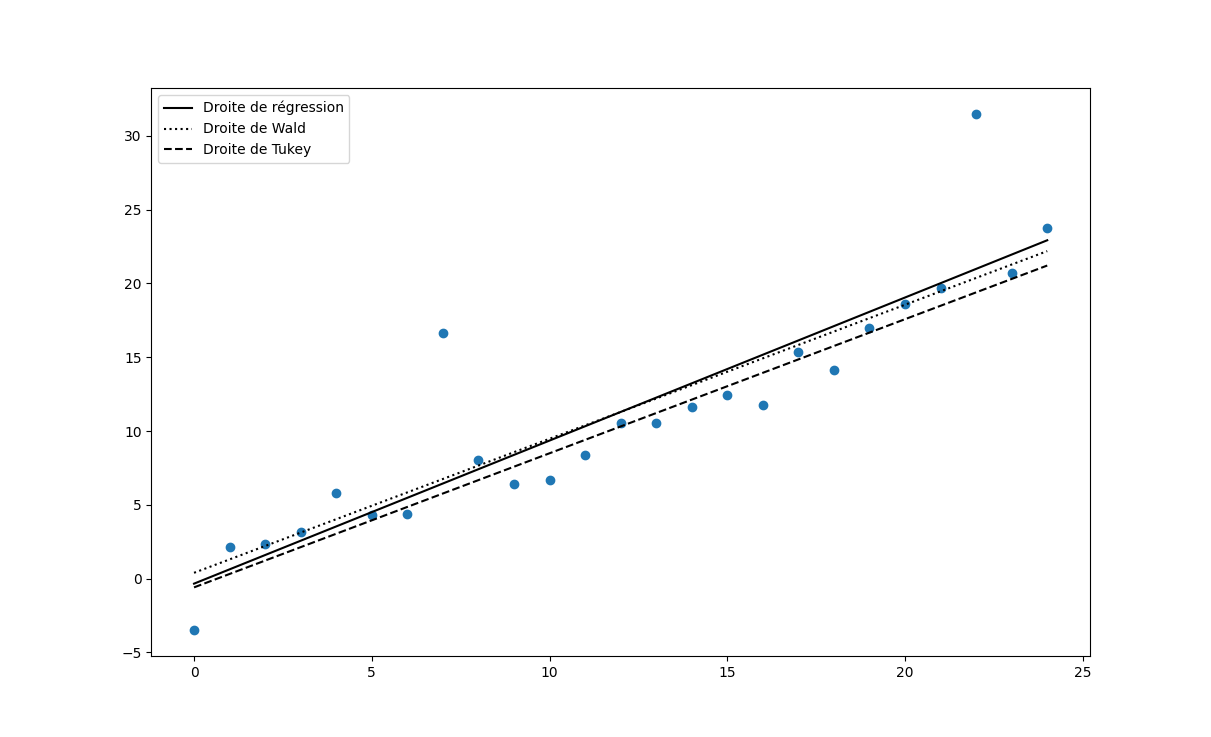
\includegraphics[width=\linewidth]{3Droites}
\caption{Exemple des 3 droites}
\end{center}
\end{figure}
%-------------------------------------------------------------------------------






